To investigate the influence of certain design parameters on the \gls{tps} a sensitivity analysis is performed. First different materials are tested using multiple lay-ups. The different lay-ups are then used to test the influence of heat flux variations on aere density. Lastly, the variations in mass due to changing radii is investigated. This investigation is done by using the tool described in Section \ref{subsec:thermaltool}.

\paragraph{\gls{tps} materials}
Table \ref{tab:tpsmatprop} shows some promising materials that can be used in the inflatable heat shield \cite{Corso2009,Corso2011,DuPont2011,Smith2011}. These materials have been proposed during the design of multiple inflatable decelerator concepts. For each material the thermal conductivity, the density, the specific heat, the maximum operative temperature and if applicable, the emissivity are given. The latter is only applicable to the top  thermal protection layers, because these layers will radiate heat into the surroundings.

\begin{table}[H]
	\caption {flexible \acrfull{tps} material properties}
	\centering
	\begin{tabular}{|l|l|l|l|l|l|l|}
		\hline
		\textbf{Material}         & \textbf{ $\mathbf{k}$ $\mathbf{\left[\frac{W}{m\cdot K}\right]} $} & \textbf{ $\mathbf{ \rho }$ $\mathbf{ \left[ \frac{kg}{m^3} \right] }$} & \textbf{  $\mathbf{ c_{p} }$ $\mathbf{ \left[ \frac{J}{kg \cdot K} \right] }$ }& \textbf{ $\mathbf{ T_{max} }$ $\mathbf{ [ K ] }$} &\textbf{ $\mathbf{ \varepsilon }$ $\mathbf{ [ - ] }$} & \textbf{Function} \\[1.6ex]   \hline \hline
		Viton       & 0.202 & 1,842 & 1,654 & N/A	 & 0.85 & radiation coating
		\\ \hline
		Nextel AF14       & 0.150                                                 & 858                                        & 1,050                                            & 1,373	 & 0.443    & rad. and heat barrier                                 \\ \hline
		Nextel BF20       & 0.146 
		& 1,362                                        & 1,130 
		& 1,643	 & 0.443  & rad. and heat barrier                                  
		\\ \hline
		Nextel XN513      & 0.148                                                 & 1,151                                       & 1,090                                            & 1,673	 & 0.443           & rad. and heat barrier                               \\ \hline
		Refrasil C1554-48 & 0.865                                                 & 924                                        & 1,172                                            & 1,533	 & 0.7     & rad. and heat barrier                                       \\ \hline
		Refrasil UC100-28 & 0.865                                                 & 890                                        & 1,172                                            & 1,255  & 0.2       & rad. and heat barrier                                    \\ \hline
		Hexcel 282 Carbon & 0.5                                                   & 891                                        & 1,000                                            & N/A 	 & 0.9      & rad. and heat barrier                                     \\ \hline
		Pyrogel 6650      & 0.030                                                 & 110                                        & 1,046                                            & 923    & ~        & insulator                                  \\ \hline
		Pyrogel 5401      & 0.0248                                                & 170                                        & 1,046                                            & N/A  	 & ~          & insulator                                 \\ \hline
		Refrasil 1800      & 0.085                                                 & 156                                        & 1,172                                            & 1,255 	 & ~           & insulator                                \\ \hline
		Refrasil 2000      & 0.095                                                 & 180                                        & 1,172                                            & 1,366 	 & ~            & insulator                               \\ \hline
		KFA 5             & 0.25                                                  & 98                                         & 1,250                                            & 1,473 	 & ~        & insulator                                   \\ \hline
		Nomex             & 0.035                                                  & 384                                         & 1,465                                            & N/A 	 & ~        & insulator                                   \\ \hline
		Kapton            & 0.12                                                  & 1,468                                       & 1,022                                            & 673	 & ~            & gas barrier                              \\ \hline
		Upilex            & 0.29                                                  & 1,470                                       & 1,130                                            & 773 	 & ~             & structural                            \\ \hline
		Kevlar            & 0.04 & 1,440                                       & 1,420                                            & 443 	 & ~             & structural                            \\ \hline
		Vectran            & 0.37 & 1,400 & 1,259 & N/A 	 &  & structural                            \\ \hline
	\end{tabular}
	\label{tab:tpsmatprop}
\end{table}

Using the same reference a selection can be made for the most promising thermal protection and insulation layers. These are Nextel BF-20 and Nicalon for the thermal protection layers. For the insulation layers these are Pyrogel 3350 and Pyrogel 6650. Using this three lay-ups are constructed in Figure \ref{fig:layersensthermal} that are tested for different heat fluxes and radii.


\begin{figure}[h]
	\centering
	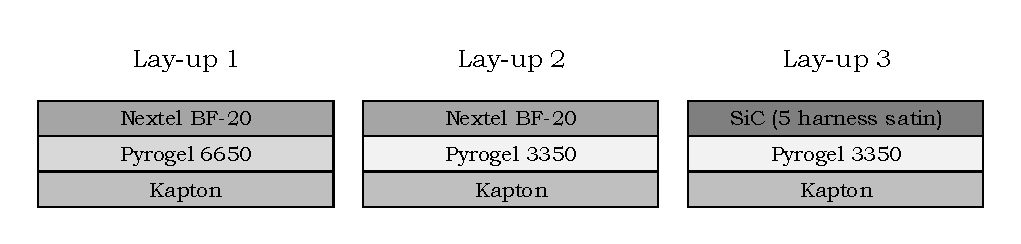
\includegraphics{./Figure/Thermal/layersensthermal.pdf}
	\caption{Tested lay-ups for the sensitivity analysis}
	\label{fig:layersensthermal}
\end{figure}

\paragraph{Effect of heat flux}
To test the effect of varying heat flux, the heat flux of an arbitrary trajectory have been multiplied to find relative values. The trajectory is found using a diameter of 12 $[m]$ and the relative factors are 0.25, 0.5, 0.75, 0.9, 1.0, 1.1, 1.4, 1.5, 2.0, 2.5 and 3.0. 

\textcolor{red}{EXTRA TEXT EN PLOTS}

\paragraph{Effect of radius}
The three lay-ups have also been tested for different radii. The aerodynamic analysis has provided heat fluxes for diameters of 6, 9, 12, 15 and 18 $[m]$. Optimising the thickness of the lay-ups for these heat flux result in Figure XX. 

\textcolor{red}{EXTRA TEXT EN PLOTS}
